\section{Results}\label{sec:results}

Fig.~\ref{fig:glance} lists the main measured quantities. We take the research questions in order.

\begin{figure*}[t]
\centering
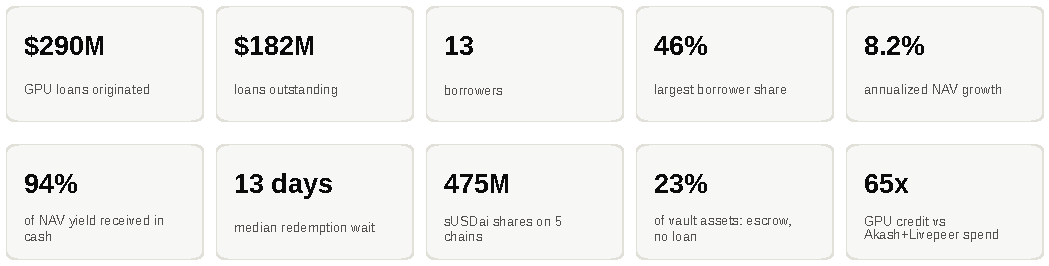
\includegraphics[width=\textwidth]{figures/fig_glance.pdf}
\caption{Key quantities at a glance, all computed from chain data over \StudyStart{} to \StudyEnd{}.}
\label{fig:glance}
\end{figure*}

\subsection{RQ1: Where the money goes}
Over the window, institutions minted \USDaiMinted{} of USDai and burned \USDaiBurned{}. Minting was backed by PYUSD, by M\textsuperscript{0}'s wrapped \$M (wM), by USDC and, marginally, by USDT (Table~\ref{tab:usdai}). Not every burn is an exit. Loan disbursements also burn USDai into the borrower's currency at origination, and the escrow redemption in Section~\ref{sec:escrow} is a burn too. Of the USDai still outstanding, most sits in the vault as idle deposit balance rather than in loans (Section~\ref{sec:recon}).

From that pool the Loan Routers originated \NLoans{} loans (excluding \NTestLoans{} test loans below \$1{,}000) for \Originated{} of principal to \NBorrowers{} distinct borrowers. \NMigrated{} loans were moved from V1 to V2 through \texttt{migrateLoan()} and are counted once. \NRepaid{} loans have been repaid in full. None has a breach or liquidation event. At \StudyEnd{}, \Outstanding{} was outstanding. Borrowers have paid \InterestPaid{} of interest, \PrincipalRepaid{} of principal and \FeesPaid{} of repayment fees. Fig.~\ref{fig:orig} shows originations by month and borrower.

\begin{figure}[t]
\centering
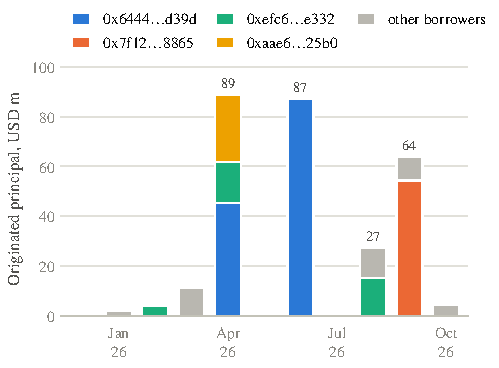
\includegraphics[width=\columnwidth]{figures/fig_originations.pdf}
\caption{Monthly originated principal by borrower. The four largest borrowers are shown separately.}
\label{fig:orig}
\end{figure}

\begin{table}[t]
\caption{USDai minting and redemption by backing asset}
\label{tab:usdai}
\centering
\footnotesize
\begin{tabular}{@{}lrr@{}}
\toprule
Backing asset & Minted & Redeemed \\
\midrule
PYUSD & \$757.72\,M & \$1,139.38\,M \\
wM (M\textsuperscript{0}) & \$542.73\,M & \$33.95\,M \\
USDC & \$353.25\,M & \$225.99\,M \\
USDT & \$0.04\,M & \$0.00\,M \\
\midrule
Total & \$1,653.7\,M & \$1,399.3\,M \\
\bottomrule
\end{tabular}

\end{table}

\subsection{What the collateral is}\label{sec:collateral}
Every loan's collateral is an ERC-721 token from the protocol's hardware contract (``USD.AI Tokenized Hardware''), either directly or wrapped in a bundle. Each token's \texttt{tokenURI}, read from the contract, points to a metadata record the protocol publishes with the server model, the number of units, a stated collateral value, a useful life and a depreciation start. We read the token IDs from every decoded \texttt{LoanTermsV2} and from the bundle wrapper's transfer logs, the URIs and owners by \texttt{eth\_call}, and the records from the protocol's host, \CollRecords{} tokens in all (retrieved \CollRetrieved{}). The records are the protocol's own statements, hosted off-chain and changeable, so what follows is what USD.AI says the collateral is, not an appraisal.

Table~\ref{tab:collateral} and Fig.~\ref{fig:collateral} list the active loans. The hardware is current generation: NVIDIA B300 and B200 servers, H200 servers and, in the small early loans, RTX 6000 and RTX 5090 workstations. Counting eight GPUs per B200, B300 and H200 server (an assumption the one press-reported loan confirms exactly, Section~\ref{sec:rq4}), the active book is secured by \CollUnits{} units carrying about \CollGPUs{} GPUs with a stated value of \CollValue{}, against \Outstanding{} outstanding: a book loan-to-value of \BookLTV{}, ranging from \LTVMin{} to \LTVMax{} by loan. Every record uses a useful life of \UsefulLife{} days, three years, with depreciation starting ``on borrow''. That is the assumption our earlier work questioned~\cite{cerron2026gpu}: at a three-year straight line, a loan at 80\% LTV is under-collateralized within eight months unless the stated value already discounts the hardware.

One token stands out. \UnpledgedName{}, \UnpledgedUnits{} servers with a stated value of \UnpledgedValue{}, secured the largest borrower's \UnpledgedPrior{} loan until that loan was repaid in full on 2026-10-01, eight days after the \EscrowOpen{} escrow deposits. The token now sits unpledged in the borrower's reserve account, and a further record for 32 GB200 NVL72 racks (\$153\,M stated) exists on the metadata host without a minted token. Read together with Section~\ref{sec:escrow}, the simplest explanation is a refinancing in progress: the old loan repaid, the new one funded through escrow but not yet originated. That does not change what holders are exposed to while it is pending, but it is the reading the protocol is most likely to give.

\begin{table}[t]
\caption{Collateral behind the active loans, from the protocol's hardware-token metadata. GPUs counted at eight per B200, B300 or H200 server; workstation units not counted.}
\label{tab:collateral}
\centering
\scriptsize
\resizebox{\columnwidth}{!}{\begin{tabular}{@{}llrrrr@{}}
\toprule
Borrower & Hardware (units) & GPUs & Stated value & Outstanding & LTV \\
\midrule
\texttt{0x7f12\ldots{}8865} & B300 (130) & 1,040 & \$77.7\,M & \$54.4\,M & 70\% \\
\texttt{0x6444\ldots{}d39d} & B200 (96) & 768 & \$42.7\,M & \$31.2\,M & 73\% \\
\texttt{0xaae6\ldots{}25b0} & B300 (72) & 576 & \$38.3\,M & \$22.4\,M & 58\% \\
\texttt{0xefc6\ldots{}e332} & B300 (34) & 272 & \$19.2\,M & \$14.9\,M & 78\% \\
\texttt{0xefc6\ldots{}e332} & H200 (75) & 600 & \$20.5\,M & \$14.1\,M & 69\% \\
\texttt{0x6444\ldots{}d39d} & B200 (32) & 256 & \$14.1\,M & \$10.5\,M & 74\% \\
\texttt{0x9243\ldots{}1960} & B300 (24) & 192 & \$12.0\,M & \$9.6\,M & 80\% \\
\texttt{0xd08f\ldots{}359a} & B200 (32) & 256 & \$14.2\,M & \$7.3\,M & 51\% \\
\texttt{0xc991\ldots{}5398} & B200 (38) & 304 & \$15.8\,M & \$7.1\,M & 45\% \\
\texttt{0xc991\ldots{}5398} & B200 (16) & 128 & \$7.1\,M & \$4.6\,M & 65\% \\
\texttt{0xefc6\ldots{}e332} & B300/RTX 6000 (27) & 72 & \$6.1\,M & \$3.4\,M & 56\% \\
\texttt{0x8db6\ldots{}2fb9} & B200 (36) & 64 & \$3.3\,M & \$1.8\,M & 54\% \\
\texttt{0x6726\ldots{}be31} & H200 (8) & 32 & \$0.9\,M & \$0.4\,M & 43\% \\
8 smaller loans & mixed (10) & n/a & \$0.97\,M & \$0.59\,M & 60\% \\
\midrule
All active & (630) & 4,560 & \$272.8\,M & \$182.2\,M & 67\% \\
\bottomrule
\end{tabular}
}
\end{table}

\begin{figure}[t]
\centering
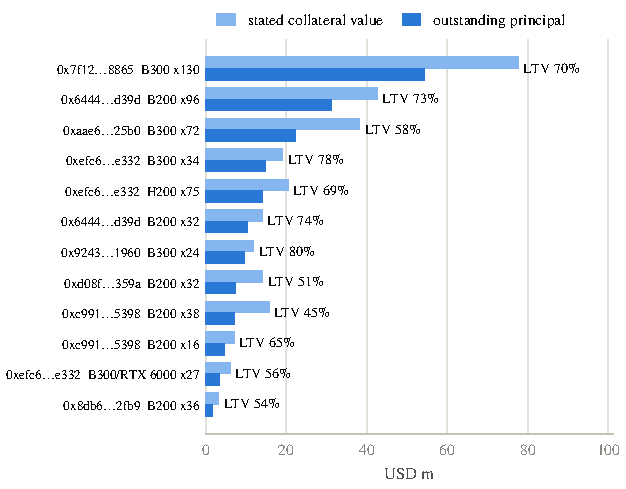
\includegraphics[width=\columnwidth]{figures/fig_collateral.pdf}
\caption{Stated collateral value against outstanding principal for the largest active loans.}
\label{fig:collateral}
\end{figure}

\subsection{Maturities and payment status}
The \NActive{} active loans have original terms of \TermMin{} to \TermMax{} years. Weighted by outstanding principal, the book has \YearsToMaturity{} years left to run: \MatTwentyEight{} matures in 2028 and \MatTwentyNine{} in 2029. Against that, holders exit through a queue with a 13-day median wait (Section~\ref{sec:queue}). Every active loan is current. The longest gap since a loan's last repayment is \MaxDaysSincePayment{} days, inside the monthly schedule, and \NLate{} loans are late. The oldest active loan is under a year old, so the book has not yet been through the part of a GPU loan's life where hardware has lost most of its value.

\subsection{RQ2: Where the yield comes from}
The deposit-side NAV of sUSDai rose from \NavStart{} to \NavEnd{} (Fig.~\ref{fig:nav}). That is \AnnTotal{} annualized over the full window and \AnnNinety{} over the last 90 days. Multiplying daily NAV changes by the outstanding share supply gives \Accrued{} of yield credited to holders.

Against that, the vault received \CashInterest{} of loan interest, \CashBase{} of base yield (net of a \AdminFee{} admin fee), \CashFees{} of origination and repayment fees, and \CashEscrow{} of escrow interest (net of the router admin fee). Cash coverage is $\kappa=$\,\CashCoverage{}. Counting only what borrowers paid (interest and fees), it is \KappaBorrowers{}. The gap is consistent with interest that accrues daily but is paid monthly, plus base yield accrued but not yet harvested. Fig.~\ref{fig:yield} shows the monthly split. Base yield was the largest cash source, at \CashBase{} against \CashInterest{} of borrower interest. Base yield has two sources, which we separate by the other events in each transaction. \CashBasePYUSD{} came from PYUSD issuer incentives harvested out of the Base Yield Escrow (a \texttt{USDai.Harvested} event in the same transaction). \CashBaseWM{} was minted from M\textsuperscript{0}'s wM, the yield-bearing stablecoin that backed USDai early on, including a single \$7.82\,M deposit on 2026-02-02. Each source on its own is smaller than borrower interest. Combined, they are more than twice as large, so over this window sUSDai holders received more cash from stablecoin issuers than from GPU borrowers.

Interest also goes to lenders other than the vault. Of the interest paid, \InterestToVault{} (\VaultInterestShare{}) went to sUSDai. \InterestToOthers{} went to two other tranche lenders: a junior tranche priced at 28\% APR and a one-unit senior position that collects repayment fees. Loans are almost entirely vault-funded (\SusdaiFunded{} of current principal).

\begin{figure}[t]
\centering
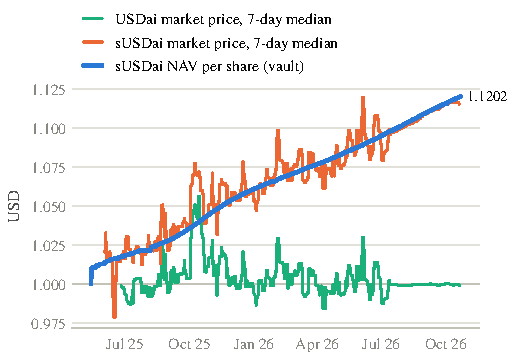
\includegraphics[width=\columnwidth]{figures/fig_nav.pdf}
\caption{sUSDai NAV per share from vault deposits and the USDai market price (GoldRush pricing).}
\label{fig:nav}
\end{figure}

\begin{figure}[t]
\centering
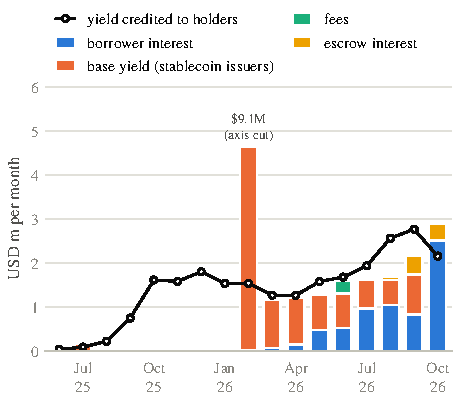
\includegraphics[width=\columnwidth]{figures/fig_yield.pdf}
\caption{Yield credited to holders (NAV growth $\times$ supply) against cash received by the vault, by month.}
\label{fig:yield}
\end{figure}

\subsection{Reconciliation with vault state}\label{sec:recon}
At block \StateBlock{} the vault reports \TotalAssets{} of assets against \TotalShares{} shares (Fig.~\ref{fig:bs}). Shares split into \HubSupply{} on Arbitrum, \BridgedSupply{} bridged out and a residual of \PendingRedeemShares{}, which the contract counts as pending redemption. Our own redemption queue shows \PendingShares{} pending, so the two differ by under 1\,M shares. Event-derived supply plus our pending queue matches \texttt{totalShares} to within \SharesGapPct{}; part of that closeness comes from offsetting small differences. The bridged supply matches the sum of the three EVM spoke snapshots plus Solana (\SpokeSolana{}). The vault's \texttt{pendingLoanBalance} is \PendingLoanBalance{}. Our stitched loan book differs from it by \LoanBookGap{} (\LoanBookGapPct{}). We take these matches as validation of the decoder, the stitching and the unit handling.

The assets side breaks down as \DepositBalance{} of idle deposit balance, \PendingLoanBalance{} of active loans, \AccruedLoanInterest{} of accrued loan interest, \BaseYieldAccrued{} of unharvested base yield, \EscrowAccrued{} of accrued escrow interest and \DTBalance{} of \texttt{depositTimelockBalance}. That last item is \DTShare{} of assets, and it is not a loan.

\begin{figure*}[t]
\centering
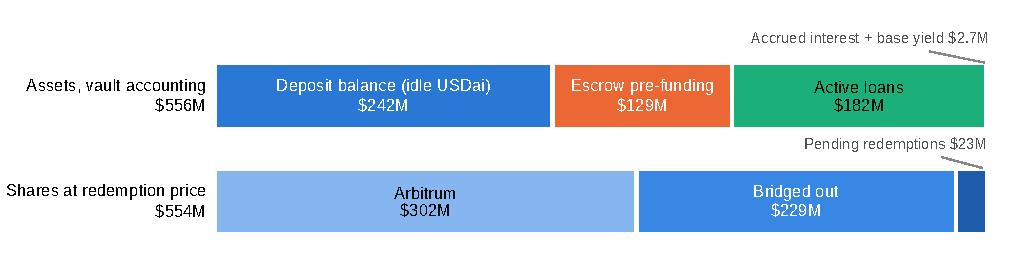
\includegraphics[width=0.9\textwidth]{figures/fig_balance_sheet.pdf}
\caption{The vault's balance sheet at block \StateBlock{}, read with \texttt{eth\_call}. Shares are valued at the redemption share price.}
\label{fig:bs}
\end{figure*}

\subsection{Checking GoldRush against the chain}\label{sec:verify}
Almost every number in this paper comes from GoldRush, so we pulled the underlying logs again from a public Arbitrum node with \texttt{eth\_getLogs}, without GoldRush, over the same block range. For each of the \NVerify{} event sets the analysis depends on, we compare the two sources log by log, identifying each log by its transaction hash, topics and data, and we compare the sum of the key amount (Table~\ref{tab:verify}). \NVerifyMatch{} of \NVerify{} sets are identical, covering \NVerifyLogs{} logs.

The check found one real problem. GoldRush's event endpoint treats \texttt{ending-block} as exclusive, so our first scan skipped the last block of every 1{,}000{,}000-block window. We confirmed this directly: a log in block $B$ is returned for the range $[B, B{+}1]$ but not for $[B, B]$. We fixed the request, fetched the 182 window-end blocks for every scanned event and re-ran the check. The patch added two Livepeer logs (one ticket payment of 0.0024 ETH) and nothing to the USD.AI events. We also found that, for some transactions, GoldRush numbers logs differently from the node, so we never match or deduplicate logs on their index.

For token supply, \texttt{totalSupply} at the snapshot block equals the sum of GoldRush holder balances exactly on Base and is 0.19\% higher on Plasma. The public Arbitrum and Ethereum nodes do not serve historical state, so there we compare against the latest block, a few hours after the snapshot, and the gaps are below 0.1\%. The escrow redemption receipt, re-read from the node, shows the same burn of 128{,}895{,}244.1 USDai and the same PYUSD payment to the same wallet. Finally, USDai itself is backed: at block \BackingBlock{} the USDai contract held \USDaiReserves{} of stablecoins (\USDaiPYUSD{} of it PYUSD) against \USDaiSupplyNow{} of USDai across the hub and the EVM spokes, a coverage of \USDaiCoverage{}. The idle deposit balance in the vault is therefore real PYUSD one redemption away, not a claim on a claim.

\begin{table}[t]
\caption{GoldRush data checked against a public Arbitrum node}
\label{tab:verify}
\centering
\scriptsize
\resizebox{\columnwidth}{!}{\begin{tabular}{@{}lrrc@{}}
\toprule
Event (Arbitrum) & RPC logs & GoldRush logs & Same \\
\midrule
Loans originated, router V1 & 35 & 35 & yes \\
Loans originated, router V2 & 6 & 6 & yes \\
Loans migrated V1 to V2 & 17 & 17 & yes \\
Loans refinanced & 3 & 3 & yes \\
Loans refinanced (3-field) & 2 & 2 & yes \\
Repayments, router V1 & 118 & 118 & yes \\
Repayments, router V2 & 79 & 79 & yes \\
Lender payouts, router V1 & 235 & 235 & yes \\
Lender payouts, router V2 & 96 & 96 & yes \\
Fees paid, router V2 & 61 & 61 & yes \\
Breaches and liquidations, V2 & 0 & 0 & yes \\
Reserve accounts created & 25 & 25 & yes \\
USDai mints & 16,348 & 16,348 & yes \\
USDai redemptions & 8,842 & 8,842 & yes \\
sUSDai deposits & 20,077 & 20,077 & yes \\
sUSDai redemption requests & 2,986 & 2,986 & yes \\
sUSDai redemptions processed & 2,841 & 2,841 & yes \\
Base yield deposited to vault & 12 & 12 & yes \\
Escrow deposits & 9 & 9 & yes \\
Escrow withdrawals & 4 & 4 & yes \\
Escrow cancellations & 3 & 3 & yes \\
Livepeer winning-ticket payments & 194,377 & 194,377 & yes \\
\midrule
\multicolumn{4}{@{}l}{\emph{sUSDai supply: \texttt{totalSupply} vs.\ sum of GoldRush holders}} \\
Arbitrum (latest block) & 270.01\,M & 270.82\,M & +0.30\% \\
Ethereum (latest block) & 101.21\,M & 101.53\,M & +0.31\% \\
Base (same block) & 3.64\,M & 3.64\,M & +0.00\% \\
Plasma (same block) & 26.16\,M & 26.11\,M & -0.19\% \\
\bottomrule
\end{tabular}
}
\end{table}

\subsection{Escrow pre-funding}\label{sec:escrow}
The vault made \NEscrow{} escrow timelock deposits totaling \EscrowDeposits{}. Most closed normally: \NEscrowClosed{} were either withdrawn into an originated loan or cancelled (\NEscrowCancelled{} cancellations, which returned principal plus interest to the vault). \NEscrowOpen{}, both made on 2026-09-23 and worth \EscrowOpen{}, carry a \texttt{loanTermsHash} that no Loan Router has originated and that has not been cancelled. Together they equal \texttt{depositTimelockBalance} to the cent. They earn an escrow rate of \EscrowAPR{}, which the vault accrues optimistically. None of the timelock contracts holds any tokens: \texttt{balanceOf} returns zero for USDai, PYUSD and USDC.

Fig.~\ref{fig:flow} and Table~\ref{tab:escrow} show where the tokens went. Every escrow deposit moves USDai from the vault to a single address we call the escrow facility (\EscrowDeposits{} in total, of which cancellations returned part). It is a Gnosis Safe, and its transactions are submitted by the same accounts that submit the protocol's own multisig transactions, so it appears to be operated by the protocol side, not by a borrower. For the two open deposits, the facility redeemed the USDai into PYUSD at the USDai contract the same day and paid the PYUSD to a single wallet we call the PYUSD hub. The hub was first active on 2026-04-29 and has 56 transactions. It also received PYUSD from the largest borrower and from the account that submits the protocol's multisig transactions. It forwarded almost everything to a high-activity wallet (off-ramp~A) that holds PYUSD and USDG and is active on 19 chains, and a smaller amount to a service wallet. The fee recipient that collects origination fees routes to the same off-ramp.

Escrow pre-funding is allowed by the contracts, and it may correspond to a signed facility whose loan has not yet been put on-chain. But from the chain's point of view, \DTBalance{} of the assets backing sUSDai is a claim that some party will later post a matching loan. The funds behind it have left the protocol's contracts, passed through a Safe run by the same operators, and moved to an off-ramp wallet. Holders are paid optimistic yield on that claim before any GPU collateral is wrapped. We describe wallets only by their on-chain roles, and the protocol should have the chance to explain the arrangement (Section~\ref{sec:disc}).

\begin{figure*}[t]
\centering
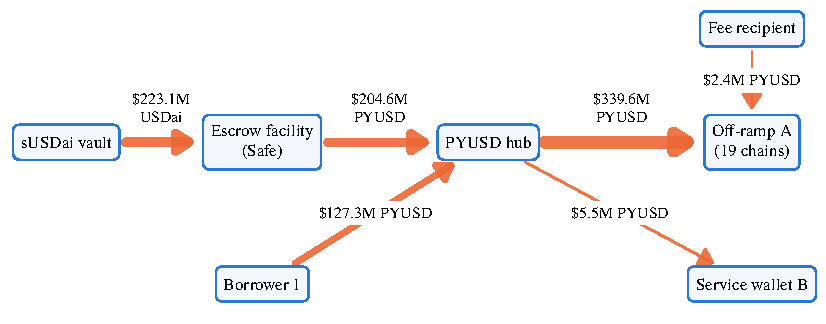
\includegraphics[width=0.92\textwidth]{figures/fig_escrow_flow.pdf}
\caption{Where escrowed vault funds went. Edge width is proportional to USD. All flows are decoded ERC-20 transfers or USDai redemptions on Arbitrum. Wallets are labeled by on-chain role only.}
\label{fig:flow}
\end{figure*}

\begin{table}[t]
\caption{Largest stablecoin flows around the escrow facility and the PYUSD hub. Hub outflows also include PYUSD the hub received from the largest borrower and the multisig submitter.}
\label{tab:escrow}
\centering
\scriptsize
\resizebox{\columnwidth}{!}{\begin{tabular}{@{}llr@{}}
\toprule
From $\rightarrow$ To & Asset & USD \\
\midrule
sUSDai vault (\texttt{0x0b2b\ldots{}5ef9}) $\rightarrow$ escrow facility & USDai & \$223.1\,M \\
PYUSD hub (\texttt{0x1168\ldots{}21b1}) $\rightarrow$ off-ramp A (\texttt{0xf845\ldots{}abb7}) & PYUSD & \$339.6\,M \\
escrow facility (\texttt{0x844b\ldots{}6286}) $\rightarrow$ PYUSD hub (\texttt{0x1168\ldots{}21b1}) & PYUSD (redeemed) & \$142.4\,M \\
escrow facility (\texttt{0x844b\ldots{}6286}) $\rightarrow$ PYUSD hub (\texttt{0x1168\ldots{}21b1}) & PYUSD & \$62.2\,M \\
escrow facility (\texttt{0x844b\ldots{}6286}) $\rightarrow$ sUSDai vault (\texttt{0x0b2b\ldots{}5ef9}) & USDai & \$16.3\,M \\
escrow facility (\texttt{0x844b\ldots{}6286}) $\rightarrow$ \texttt{0x24a9\ldots{}1392} & PYUSD & \$6.0\,M \\
escrow facility (\texttt{0x844b\ldots{}6286}) $\rightarrow$ \texttt{0xfd1c\ldots{}ca91} & USDai & \$5.9\,M \\
\texttt{0xfd1c\ldots{}ca91} $\rightarrow$ PYUSD hub (\texttt{0x1168\ldots{}21b1}) & PYUSD (redeemed) & \$5.9\,M \\
PYUSD hub (\texttt{0x1168\ldots{}21b1}) $\rightarrow$ service wallet B (\texttt{0x264b\ldots{}97b5}) & PYUSD & \$5.5\,M \\
escrow facility (\texttt{0x844b\ldots{}6286}) $\rightarrow$ \texttt{0x6034\ldots{}23ef} & USDai & \$5.1\,M \\
\bottomrule
\end{tabular}
}
\end{table}

\subsection{RQ3 and RQ6: Holders and the cross-chain footprint}
On Arbitrum, sUSDai has \ArbHolders{} holders. The largest holds \ArbTopOne{} and the top ten hold \ArbTopTen{} (HHI \ArbHHI{}, Gini \ArbGini{}). Table~\ref{tab:holders} gives the same statistics for each chain, and Table~\ref{tab:top} lists the largest hub holders with the contract labels GoldRush returns. On every chain, a handful of contracts and pools hold most of the supply (Fig.~\ref{fig:conc}). The largest DeFi venue is Pendle, which holds \PendleArb{} of Arbitrum sUSDai. On Plasma, \PendlePlasmaUSDai{} of USDai sits in Pendle and another \VaultPlasmaUSDai{} in vault strategies, so most of that chain's supply is in yield-trading and looping positions rather than in wallets.

Supply is spread across five chains: \SharesArb{} on Arbitrum, \SharesEth{} on Ethereum, \SharesPlasma{} on Plasma, \SharesBase{} on Base and \SolanaShares{} on Solana (Fig.~\ref{fig:supply}). Only one address holds at least \CrossChainMin{} sUSDai on more than one EVM chain. It is a high-activity contract with more than 8 million Arbitrum transactions, and it is the largest or second-largest holder on all four EVM chains, with \(>\)95\% of supply on Base and Plasma. Historical snapshots at monthly blocks show when the Ethereum footprint appeared. sUSDai on Ethereum was a test-sized position (\EthHoldersFirst{} holders in \EthHistFirst{}, under 0.1\,M shares on 2026-06-01) until mid-2026. It then grew to \EthSupplyLast{} shares and \EthHoldersLast{} holders by \EthHistLast{} (Fig.~\ref{fig:ethhist}). Two addresses hold \EthTopTwo{} of it: the cross-chain contract above and the Morpho Blue singleton (\EthMorpho{}), where sUSDai is posted as loan collateral. GoldRush's cross-chain activity endpoint shows where borrowers and top holders operate (Fig.~\ref{fig:activity}). The \ActBorrowers{} borrowers with activity data have used between \BorrChainsMin{} and \BorrChainsMax{} chains (median \BorrChainsMed{}), so borrowers are active well beyond Arbitrum. The \ActHolders{} top holders range from \HoldChainsMin{} to \HoldChainsMax{} chains (median \HoldChainsMed{}). Many single-chain holders are pools and vault contracts.

\begin{table}[t]
\caption{sUSDai holder concentration by chain}
\label{tab:holders}
\centering
\footnotesize
\begin{tabular}{@{}lrrrrr@{}}
\toprule
Chain & Holders & Supply & Top-1 & Top-10 & HHI \\
\midrule
Arbitrum & 3,778 & 270.8\,M & 33.3\% & 86.7\% & 0.209 \\
Base & 468 & 3.6\,M & 95.1\% & 99.6\% & 0.905 \\
Ethereum & 135 & 101.5\,M & 81.6\% & 100.0\% & 0.699 \\
Plasma & 1,424 & 26.1\,M & 97.6\% & 99.9\% & 0.953 \\
\bottomrule
\end{tabular}

\end{table}

\begin{table}[t]
\caption{Largest sUSDai holders on Arbitrum}
\label{tab:top}
\centering
\scriptsize
\begin{tabular}{@{}lrrl@{}}
\toprule
Holder & sUSDai & Share & Label \\
\midrule
\texttt{0x7ced\ldots{}20af} & 90.16\,M & 33.3\% & unlabeled \\
\texttt{0x52aa\ldots{}e497} & 75.43\,M & 27.9\% & unlabeled \\
\texttt{0x30cc\ldots{}2f62} & 35.68\,M & 13.2\% & SY Staked USDai \\
\texttt{0xed41\ldots{}6029} & 8.89\,M & 3.3\% & unlabeled \\
\texttt{0xe7f5\ldots{}e8e2} & 6.60\,M & 2.4\% & unlabeled \\
\texttt{0x9167\ldots{}6700} & 5.38\,M & 2.0\% & unlabeled \\
\texttt{0xbeed\ldots{}6dba} & 4.56\,M & 1.7\% & unlabeled \\
\texttt{0xa520\ldots{}a575} & 2.82\,M & 1.0\% & unlabeled \\
\bottomrule
\end{tabular}

\end{table}

\begin{figure}[t]
\centering
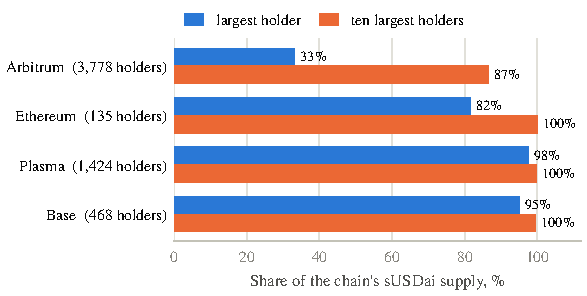
\includegraphics[width=\columnwidth]{figures/fig_concentration.pdf}
\caption{Share of each chain's sUSDai held by its largest holder and its ten largest holders.}
\label{fig:conc}
\end{figure}

\begin{figure}[t]
\centering
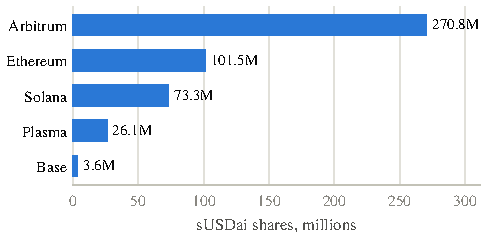
\includegraphics[width=\columnwidth]{figures/fig_supply.pdf}
\caption{sUSDai shares by chain (holder snapshots; Solana from mint supply).}
\label{fig:supply}
\end{figure}

\begin{figure}[t]
\centering
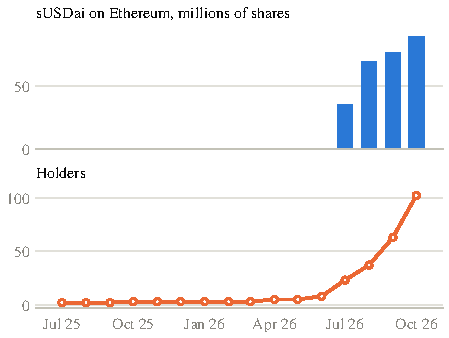
\includegraphics[width=\columnwidth]{figures/fig_eth_holders.pdf}
\caption{sUSDai on Ethereum over time, from historical holder snapshots at the first block of each month.}
\label{fig:ethhist}
\end{figure}

\begin{figure*}[t]
\centering
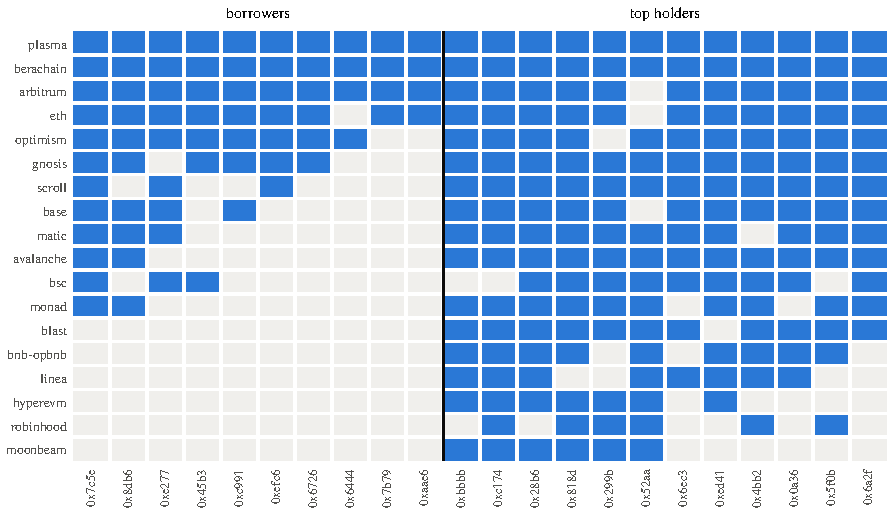
\includegraphics[width=\textwidth]{figures/fig_activity.pdf}
\caption{Cross-chain activity of borrowers and top holders from GoldRush's address activity endpoint. Each filled cell is a chain on which the address has transacted.}
\label{fig:activity}
\end{figure*}

\subsection{RQ4: Borrower concentration}\label{sec:rq4}
The loan book is concentrated. The largest borrower accounts for \TopOneShare{} of originations and the top three for \TopThreeShare{}. HHI is \HHIOrig{} on originations and \HHIOut{} on outstanding principal. Both are above 0.18, the threshold for a highly concentrated market in the 2023 U.S. Merger Guidelines. Table~\ref{tab:borrowers} lists each borrower. Rates run from \RateMin{} to \RateMax{}, with an outstanding-weighted average of \RateWavg{}. \NReserveAccounts{} reserve accounts map back to borrowers through the factory. Press coverage names some borrowers. One reported \$26.82\,M facility, secured by 576 NVIDIA B300 GPUs~\cite{blockmedia2026}, matches, to the reported precision, a single loan of \$26{,}821{,}644 originated on 2026-04-06, and its collateral record lists 72 B300 servers, which at eight GPUs per server is the same 576. We do not attribute any address to an off-chain entity in our results.

\begin{table}[t]
\caption{Borrowers (address prefixes), sorted by originated principal}
\label{tab:borrowers}
\centering
\scriptsize
\begin{tabular}{@{}lrrrr@{}}
\toprule
Borrower & Loans & Originated & Outstanding & Interest paid \\
\midrule
\texttt{0x6444\ldots{}d39d} & 3 & \$132.40\,M & \$41.71\,M & \$2,995\,k \\
\texttt{0x7f12\ldots{}8865} & 1 & \$54.40\,M & \$54.40\,M & \$356\,k \\
\texttt{0xefc6\ldots{}e332} & 3 & \$36.01\,M & \$32.42\,M & \$1,373\,k \\
\texttt{0xaae6\ldots{}25b0} & 1 & \$26.82\,M & \$22.35\,M & \$1,123\,k \\
\texttt{0xc991\ldots{}5398} & 3 & \$18.93\,M & \$11.70\,M & \$585\,k \\
\texttt{0x9243\ldots{}1960} & 1 & \$9.56\,M & \$9.56\,M & \$58\,k \\
\texttt{0xd08f\ldots{}359a} & 1 & \$7.50\,M & \$7.32\,M & \$121\,k \\
\texttt{0x8db6\ldots{}2fb9} & 1 & \$2.30\,M & \$1.79\,M & \$206\,k \\
\texttt{0xe277\ldots{}0eb9} & 7 & \$0.54\,M & \$0.43\,M & \$39\,k \\
\texttt{0x6726\ldots{}be31} & 1 & \$0.53\,M & \$0.40\,M & \$31\,k \\
\texttt{0x7c5e\ldots{}854e} & 1 & \$0.48\,M & \$0.00\,M & \$23\,k \\
\texttt{0x7b79\ldots{}4462} & 15 & \$0.44\,M & \$0.00\,M & \$15\,k \\
\texttt{0x45b3\ldots{}94d3} & 1 & \$0.20\,M & \$0.16\,M & \$15\,k \\
\bottomrule
\end{tabular}

\end{table}

\subsection{RQ5: Redemptions and GPU prices}\label{sec:queue}
Holders filed \NRedeemRequests{} redemption requests from \NRedeemers{} addresses, for \RequestedShares{} shares. The median completed request waited \WaitMedian{} days, the 90th percentile \WaitPNinety{} days, and the longest \WaitMax{} days. \PendingShares{} shares are still in the queue. Servicing is lumpy (Fig.~\ref{fig:queue}): the queue is cleared in a small number of large batches. Three servicing calls on 2026-03-07 and 2026-04-06 together paid out about \$217\,M. Priced in PYUSD, which removes feed noise common to both tokens, USDai never traded below \USDaiRatioMin{} (on \USDaiRatioMinDate{}). Selling on a DEX is the only alternative to waiting.

We find no useful relationship between requests and GPU rental prices. Over \GPUWeeks{} overlapping weeks, Spearman's $\rho$ between weekly requested shares and the H100 rental price is \RhoLevel{} in levels and \RhoChange{} in weekly changes (Fig.~\ref{fig:redgpu}). The level correlation reflects two trends: redemptions grew as the protocol grew, while rental prices fell. It is not evidence that holders react to GPU prices.

\begin{figure}[t]
\centering
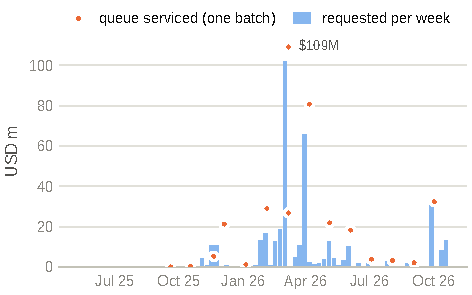
\includegraphics[width=\columnwidth]{figures/fig_queue.pdf}
\caption{Weekly redemption requests (USD at NAV) and queue servicing batches.}
\label{fig:queue}
\end{figure}

\begin{figure}[t]
\centering
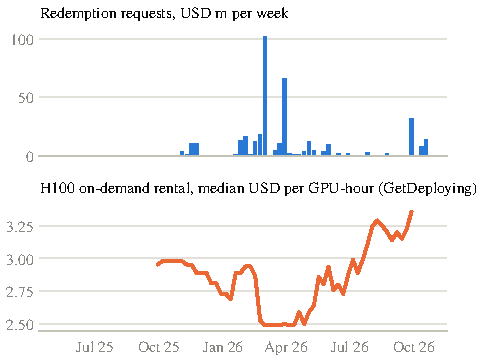
\includegraphics[width=\columnwidth]{figures/fig_redemptions.pdf}
\caption{Weekly redemption requests against the median H100 on-demand rental price (GetDeploying).}
\label{fig:redgpu}
\end{figure}

\subsection{RQ7: GPU credit versus realized compute demand}
Over the same window, Livepeer gateways paid orchestrators \LPETH{} ETH (\LPUSD{}) in \LPTickets{} winning tickets. \LPGateways{} gateways paid \LPOrchestrators{} orchestrators. The largest gateway accounts for \LPTopGateway{} of payments and the top three for \LPTopThree{} (HHI \LPHHIG{}). On the supply side, payments are spread out (HHI \LPHHIO{}). Livepeer's payments mix video transcoding and AI inference, and the events do not separate the two.

Akash, measured through its own API, recorded \AKUSD{} of spend in the window and \AKAllTime{} all-time. Active leased GPUs ranged from \AKGPUMin{} to \AKGPUMax{}. On \AKRetrieved{}, the network reported \AKGPUNow{} of \AKGPUTotal{} GPUs active across \AKProviders{} providers (Fig.~\ref{fig:akash}). The median Akash H100 price was \AKHundred{}/hr and the A100 \AKAHundred{}/hr, against a centralized-cloud H100 median of \CentralH{}/hr (Fig.~\ref{fig:prices}).

Fig.~\ref{fig:markets} and Table~\ref{tab:markets} put the three side by side on a log scale. GPU credit lent through one on-chain vault is about \CreditMultiple{} times all compute bought and settled on these two established decentralized compute markets combined (\ComputeSpend{}). Demand is concentrated on both sides of the comparison: USD.AI borrowers have an HHI of \HHIOrig{} and Livepeer gateways \LPHHIG{}, while Livepeer's supply side is far more spread out (Fig.~\ref{fig:lmk}). None of the GPU use that these loans finance appears on-chain.

\subsection{What the debt implies about the compute}\label{sec:implied}
The chain does not show the GPUs, but it shows what they have to earn. Each active loan has an outstanding principal, a fixed rate and a maturity, so the annual debt service is known: \DebtInterest{} of interest plus \DebtAmort{} of principal if the loans amortize straight-line to maturity, \DebtService{} in all. Our earlier work treated machine labor as hours of work rather than units of hardware~\cite{liquidlabor,cerron2026gpu}; the same frame turns this debt into GPU-hours. At the Akash H100 median of \AKHundred{} per hour, the borrowers must sell \GPUhAkashPrice{}\,M GPU-hours a year to service the debt from rental revenue alone. At 70\% utilization that is \GPUsAkashPrice{} H100s running all year, drawing about \MWAkashPrice{}\,MW at 1.5\,kW per GPU before cooling. At the centralized-cloud price of \CentralH{} it is \GPUsCentralPrice{} GPUs (\MWCentralPrice{}\,MW); at \$1.50, the low end of 2025 spot pricing~\cite{friedman2025}, it is \GPUsLowPrice{} (\MWLowPrice{}\,MW). Fig.~\ref{fig:implied} shows the curve. For scale, the entire Akash network has \AKGPUTotal{} GPUs. This is a lower bound: it ignores the borrowers' power, staff and data-center costs, and it assumes rental income is the only source of repayment. The pledged fleet is about \CollGPUs{} GPUs (Section~\ref{sec:collateral}), so at 70\% utilization it covers debt service at \Breakeven{} per GPU-hour and at full utilization at \BreakevenFull{}. Those are B200 and B300 class parts, which rent above H100 rates today, so the fleet can carry the debt if it is rented; the margin is thinner than it looks, because the price has to cover power and operations as well, and the stated collateral value already assumes a three-year life.

The number is testable because the pledge is published. What is not published is utilization, rental revenue or the location and power contract of the hardware. A borrower that posted those would be the first a lender could underwrite from the chain alone.

\begin{figure}[t]
\centering
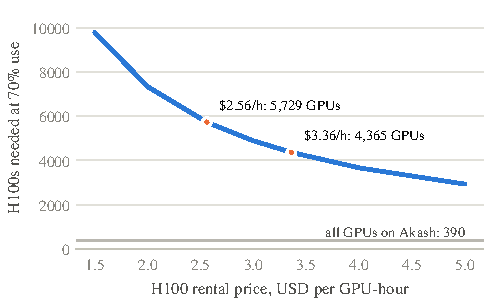
\includegraphics[width=\columnwidth]{figures/fig_implied_gpus.pdf}
\caption{H100s that must run at 70\% utilization to service the outstanding debt from rental revenue, as a function of the rental price. The Akash network's total GPU count is shown for scale.}
\label{fig:implied}
\end{figure}

\begin{figure}[t]
\centering
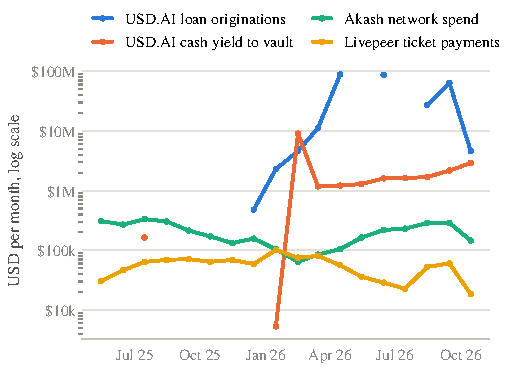
\includegraphics[width=\columnwidth]{figures/fig_markets.pdf}
\caption{Monthly USD volume: USD.AI originations and cash yield, Akash spend and Livepeer ticket payments (log scale).}
\label{fig:markets}
\end{figure}

\begin{figure}[t]
\centering
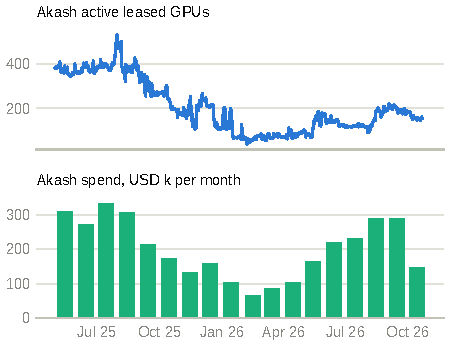
\includegraphics[width=\columnwidth]{figures/fig_akash.pdf}
\caption{Akash active leased GPUs and monthly spend (Akash Console API).}
\label{fig:akash}
\end{figure}

\begin{figure}[t]
\centering
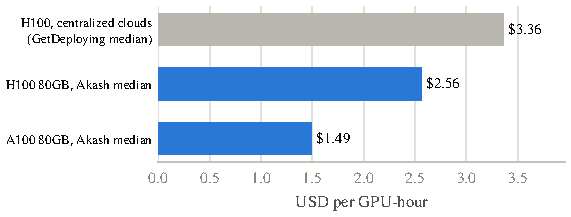
\includegraphics[width=\columnwidth]{figures/fig_gpu_prices.pdf}
\caption{GPU rental prices: decentralized (Akash median) and centralized (GetDeploying median), USD per GPU-hour.}
\label{fig:prices}
\end{figure}

\begin{figure}[t]
\centering
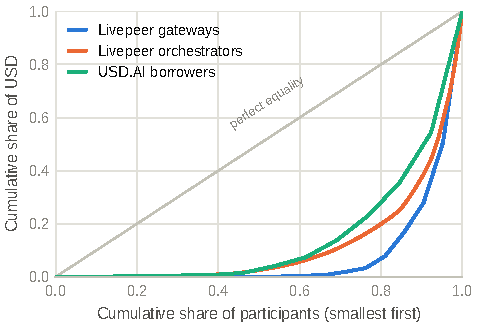
\includegraphics[width=\columnwidth]{figures/fig_lorenz_markets.pdf}
\caption{Concentration of payers and payees: Livepeer gateways and orchestrators against USD.AI borrowers.}
\label{fig:lmk}
\end{figure}

\begin{table}[t]
\caption{GPU credit and decentralized compute, study window}
\label{tab:markets}
\centering
\scriptsize
\resizebox{\columnwidth}{!}{\begin{tabular}{@{}lrrr@{}}
\toprule
Metric (study window) & USD.AI & Akash & Livepeer \\
\midrule
USD volume & \$290.1\,M lent & \$3.46\,M spent & \$1.01\,M paid \\
Revenue to capital/providers & \$6.94\,M interest & \$3.46\,M & \$1.01\,M \\
Demand-side counterparties & 13 borrowers & n/a & 21 gateways \\
Supply-side counterparties & 4 tranche lenders & 58 providers & 104 orchestrators \\
Top-1 share & 45.6\% & n/a & 49.4\% \\
Data source & GoldRush (Arbitrum) & Akash Console API & GoldRush (Arbitrum) \\
\bottomrule
\end{tabular}
}
\end{table}
